%
% graphisch2.tex
%
% (c) 2020 Prof Dr Andreas Müller, Hochschule Rapperswil
%
\begin{figure}
\centering
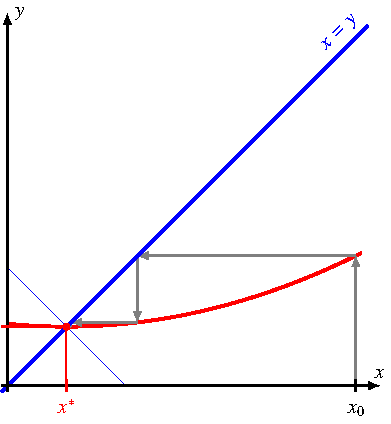
\includegraphics{chapters/10-arithmetik/figures/quadratisch.pdf}
\caption{Die Fixpunktiteration $x_{n+1}=f(x_n)$ konvergiert quadratisch
gegen den Fixpunkt $x^*$
für $f'(x^*)=0$.
\label{buch:figure:fixpunkt:quadratisch}}
\end{figure}
